\PassOptionsToPackage{unicode=true}{hyperref} % options for packages loaded elsewhere
\PassOptionsToPackage{hyphens}{url}
%
\documentclass[12pt,oneside]{krantz}
\usepackage{lmodern}
\usepackage{amssymb,amsmath}
\usepackage{ifxetex,ifluatex}
\usepackage{fixltx2e} % provides \textsubscript
\ifnum 0\ifxetex 1\fi\ifluatex 1\fi=0 % if pdftex
  \usepackage[T1]{fontenc}
  \usepackage[utf8]{inputenc}
  \usepackage{textcomp} % provides euro and other symbols
\else % if luatex or xelatex
  \usepackage{unicode-math}
  \defaultfontfeatures{Ligatures=TeX,Scale=MatchLowercase}
\fi
% use upquote if available, for straight quotes in verbatim environments
\IfFileExists{upquote.sty}{\usepackage{upquote}}{}
% use microtype if available
\IfFileExists{microtype.sty}{%
\usepackage[]{microtype}
\UseMicrotypeSet[protrusion]{basicmath} % disable protrusion for tt fonts
}{}
\IfFileExists{parskip.sty}{%
\usepackage{parskip}
}{% else
\setlength{\parindent}{0pt}
\setlength{\parskip}{6pt plus 2pt minus 1pt}
}
\usepackage{hyperref}
\hypersetup{
            pdftitle={Kitty's Story},
            pdfauthor={by Beckett and Felix},
            pdfborder={0 0 0},
            breaklinks=true}
\urlstyle{same}  % don't use monospace font for urls
\usepackage{longtable,booktabs}
% Fix footnotes in tables (requires footnote package)
\IfFileExists{footnote.sty}{\usepackage{footnote}\makesavenoteenv{longtable}}{}
\usepackage{graphicx,grffile}
\makeatletter
\def\maxwidth{\ifdim\Gin@nat@width>\linewidth\linewidth\else\Gin@nat@width\fi}
\def\maxheight{\ifdim\Gin@nat@height>\textheight\textheight\else\Gin@nat@height\fi}
\makeatother
% Scale images if necessary, so that they will not overflow the page
% margins by default, and it is still possible to overwrite the defaults
% using explicit options in \includegraphics[width, height, ...]{}
\setkeys{Gin}{width=\maxwidth,height=\maxheight,keepaspectratio}
\setlength{\emergencystretch}{3em}  % prevent overfull lines
\providecommand{\tightlist}{%
  \setlength{\itemsep}{0pt}\setlength{\parskip}{0pt}}
\setcounter{secnumdepth}{5}
% Redefines (sub)paragraphs to behave more like sections
\ifx\paragraph\undefined\else
\let\oldparagraph\paragraph
\renewcommand{\paragraph}[1]{\oldparagraph{#1}\mbox{}}
\fi
\ifx\subparagraph\undefined\else
\let\oldsubparagraph\subparagraph
\renewcommand{\subparagraph}[1]{\oldsubparagraph{#1}\mbox{}}
\fi

% set default figure placement to htbp
\makeatletter
\def\fps@figure{htbp}
\makeatother

\usepackage{booktabs}
\usepackage{caption}
\captionsetup[figure]{labelformat=empty}
\usepackage[]{natbib}
\bibliographystyle{plainnat}

\title{Kitty's Story}
\providecommand{\subtitle}[1]{}
\subtitle{A New Series}
\author{by Beckett and Felix}
\date{2019-01-26}

\begin{document}
\maketitle

{
\setcounter{tocdepth}{1}
\tableofcontents
}
\hypertarget{preface}{%
\chapter*{Preface}\label{preface}}


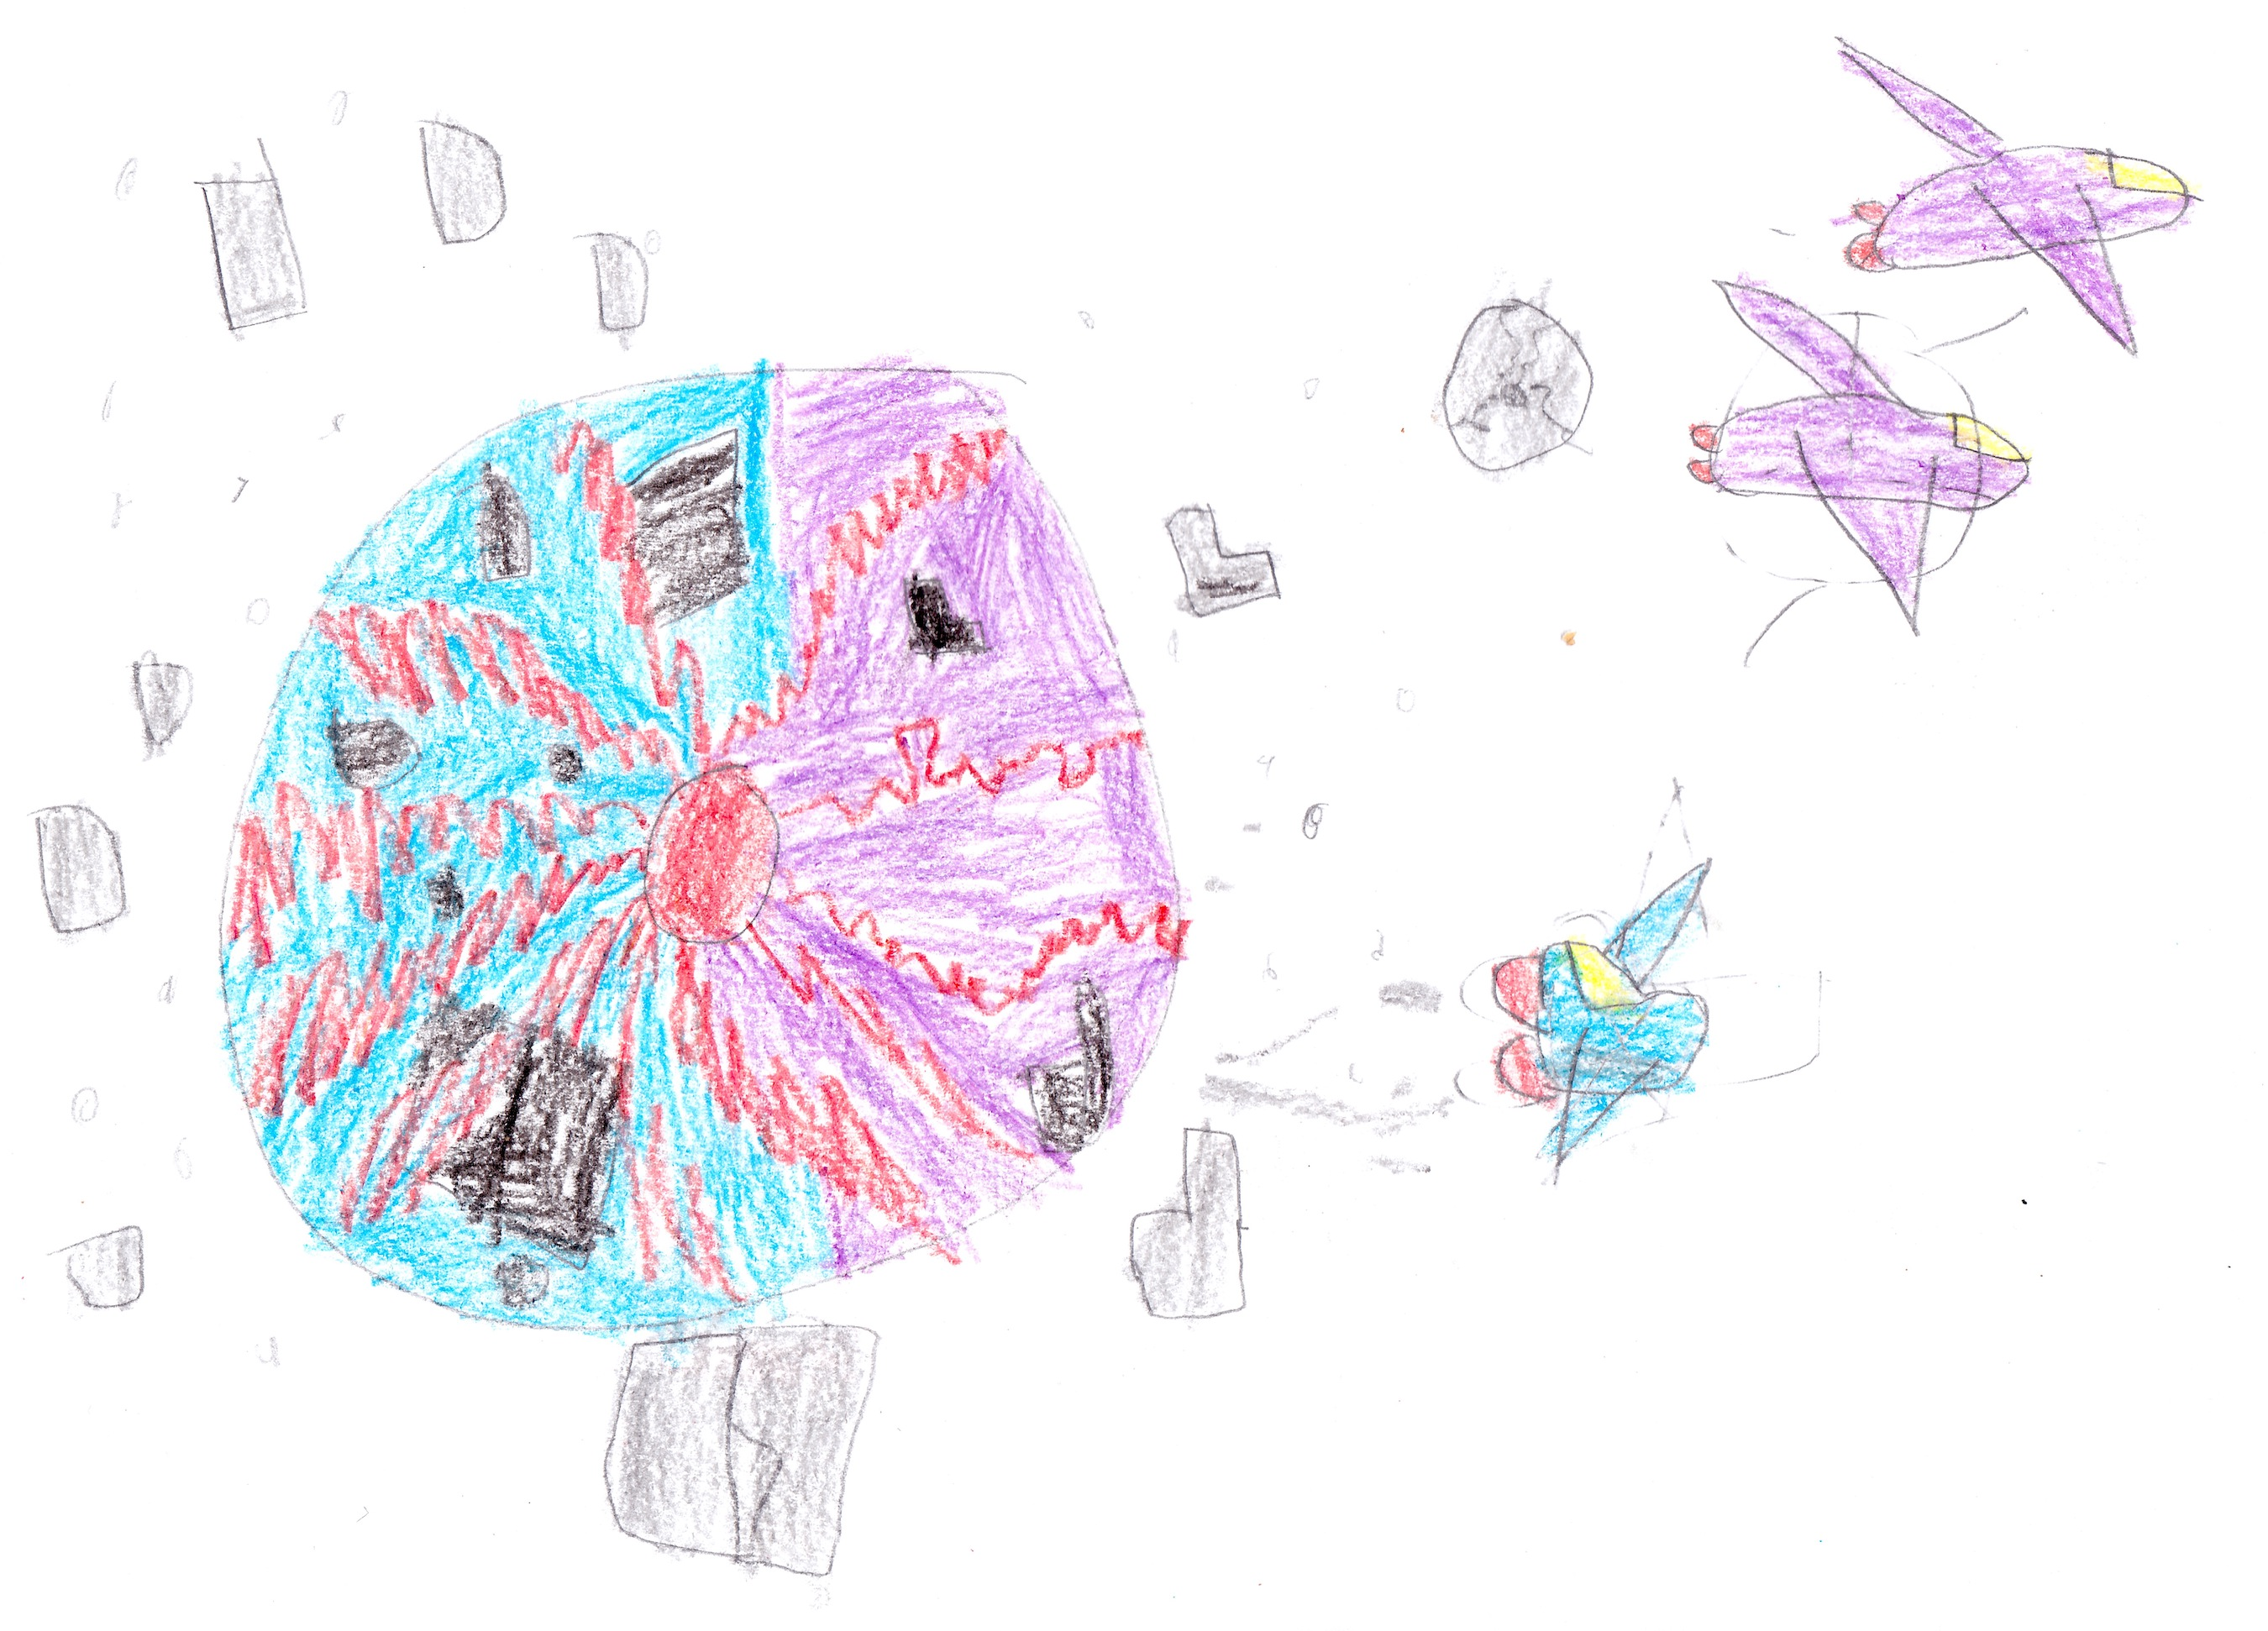
\includegraphics{img/catplanet.jpg}

We wanted to do something different in this book. I wanted to do a joint
work with my brother, Felix, so I had the idea of writing a book about
his stuff cat, Kitty. Felix came up with with the story about Cat
Planet. It was natural for me to write down the story and then have
Felix color the pictures. This was a fun collaboration, and we're
already planning the next book in the series. We hope you enjoy this new
series.

\hypertarget{about-the-authors}{%
\chapter*{About the Authors}\label{about-the-authors}}


Beckett is an aspiring author and illustrator. Beckett also loves
Minecraft, Lego's, and Transformers, as well as making up endless
stories while he walks.

Felix loves to draw. When he isn't coloring Felix likes to play Lego's
and transformers. He also loves cats because they make him feel happy.
He has a stuffed animal named Kitty.

\hypertarget{acknowledgements}{%
\chapter*{Acknowledgements}\label{acknowledgements}}


Thanks to Dad for helping us publish this book online.

\hypertarget{king-cat}{%
\chapter{King cat}\label{king-cat}}

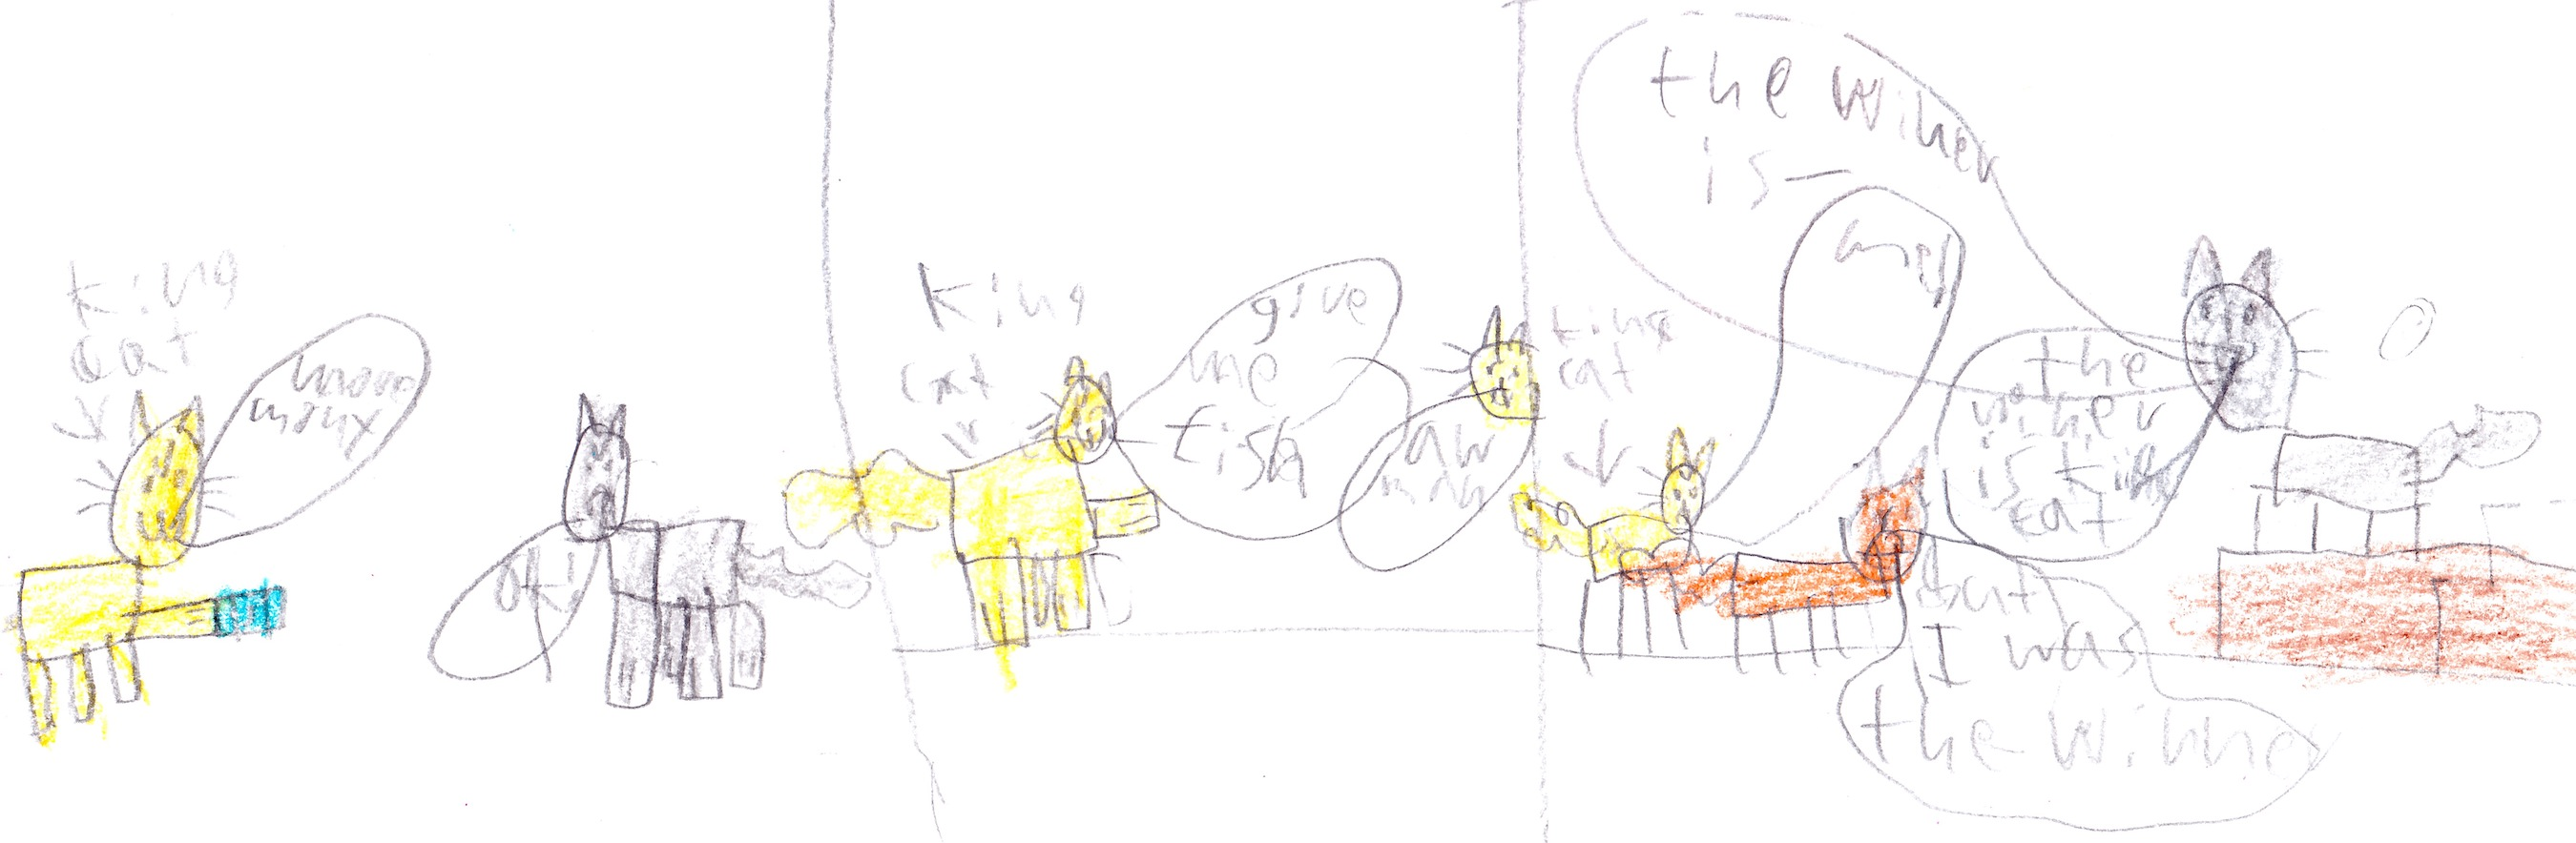
\includegraphics{img/thewinner.jpg}

Once there was a king on Cat Planet named King Cat. He was a mean king.
He got all the fish, money, and prizes. King Cat was happy even when a
cat lost. He gave himself a prize because he said so.

\hypertarget{kitty}{%
\chapter{Kitty}\label{kitty}}

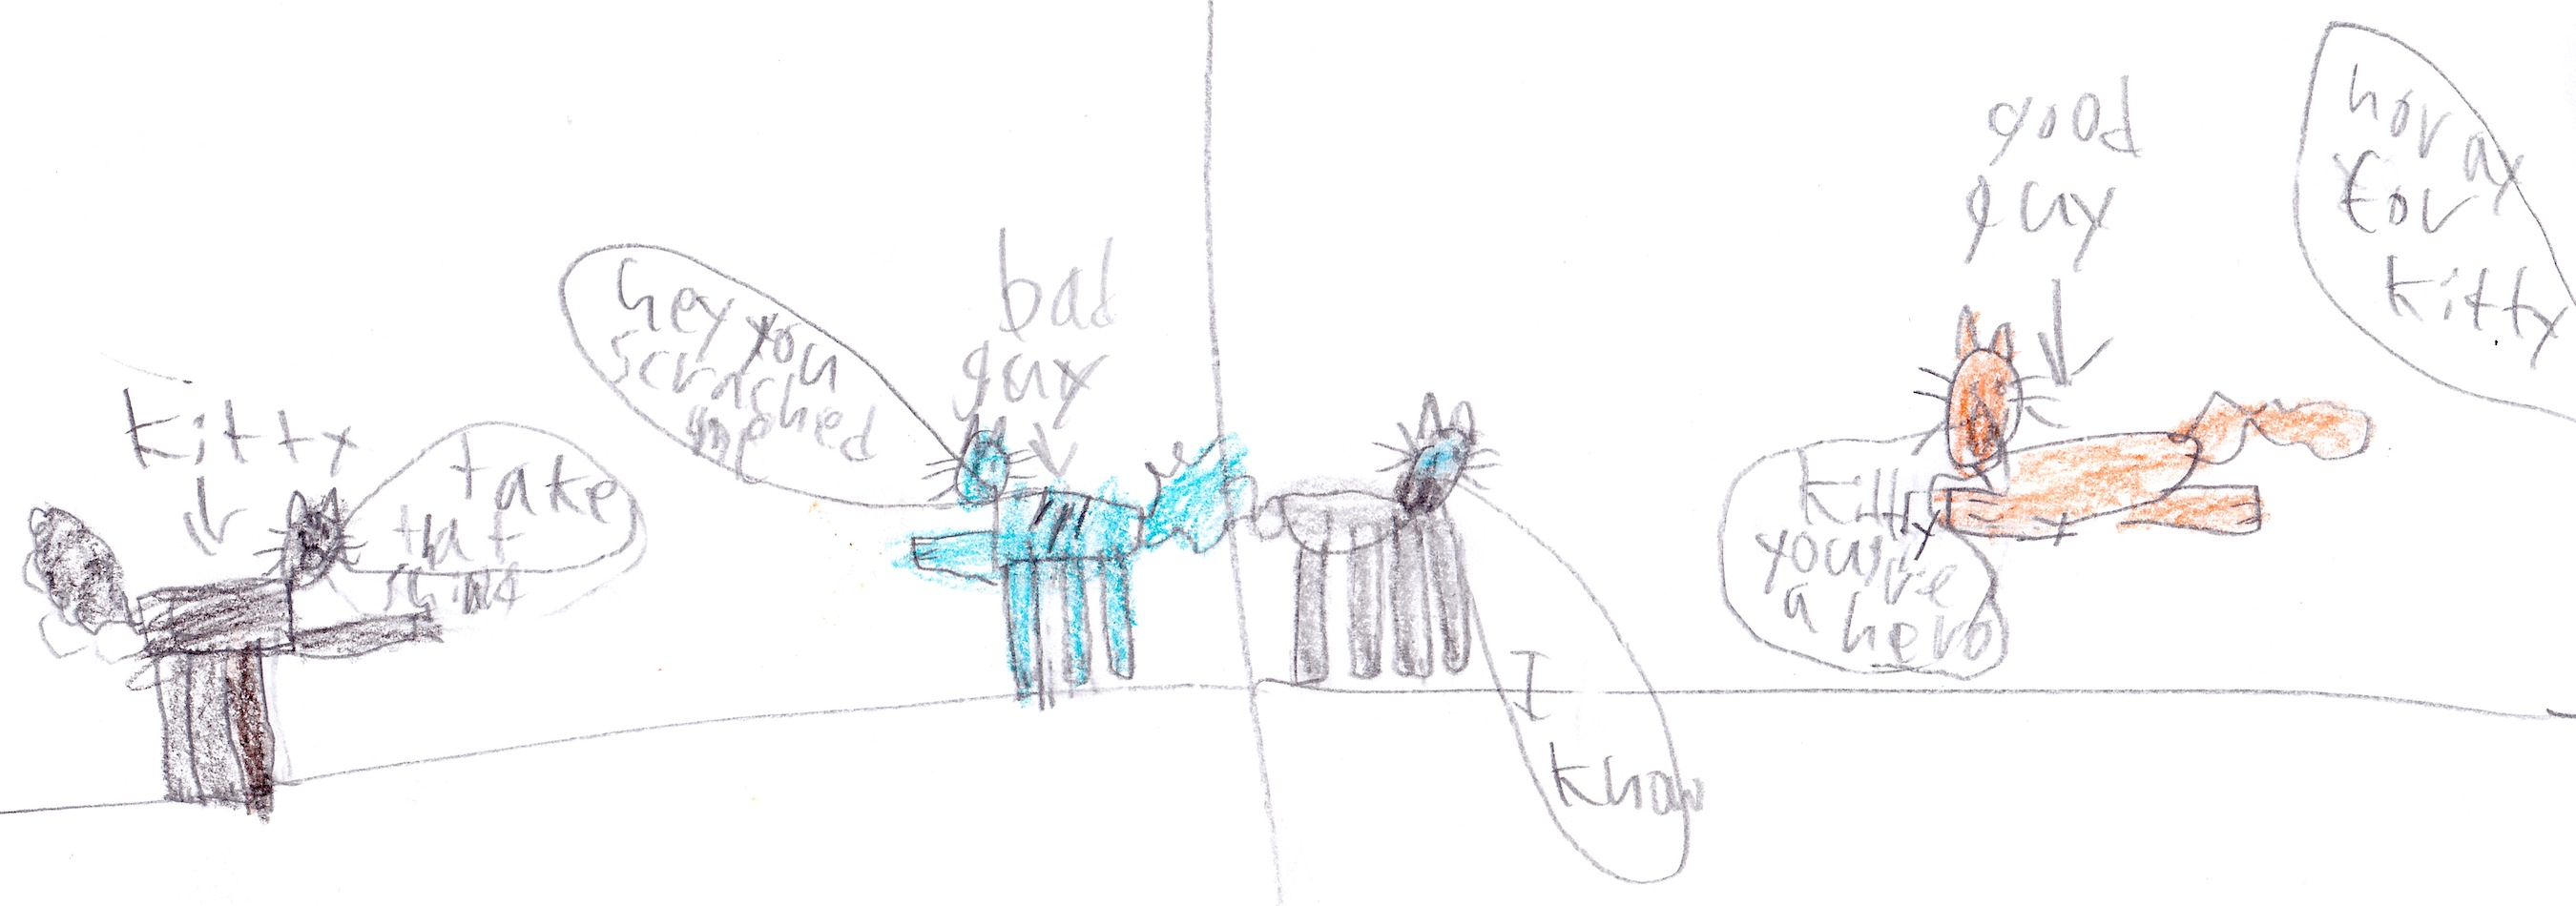
\includegraphics{img/kittyhero.jpg}

Kitty was a warrior. He fought battles all over Cat Planet. Kitty was
known for his great skill and good deeds and never giving up. He got no
fish, money, or prizes, but he did get famous. That was enough to keep
him happy and proud. Kitty was also very nice. You might think King Cat
hates Kitty and you would be right.

\hypertarget{mr-fluffy-pants}{%
\chapter{Mr Fluffy Pants}\label{mr-fluffy-pants}}

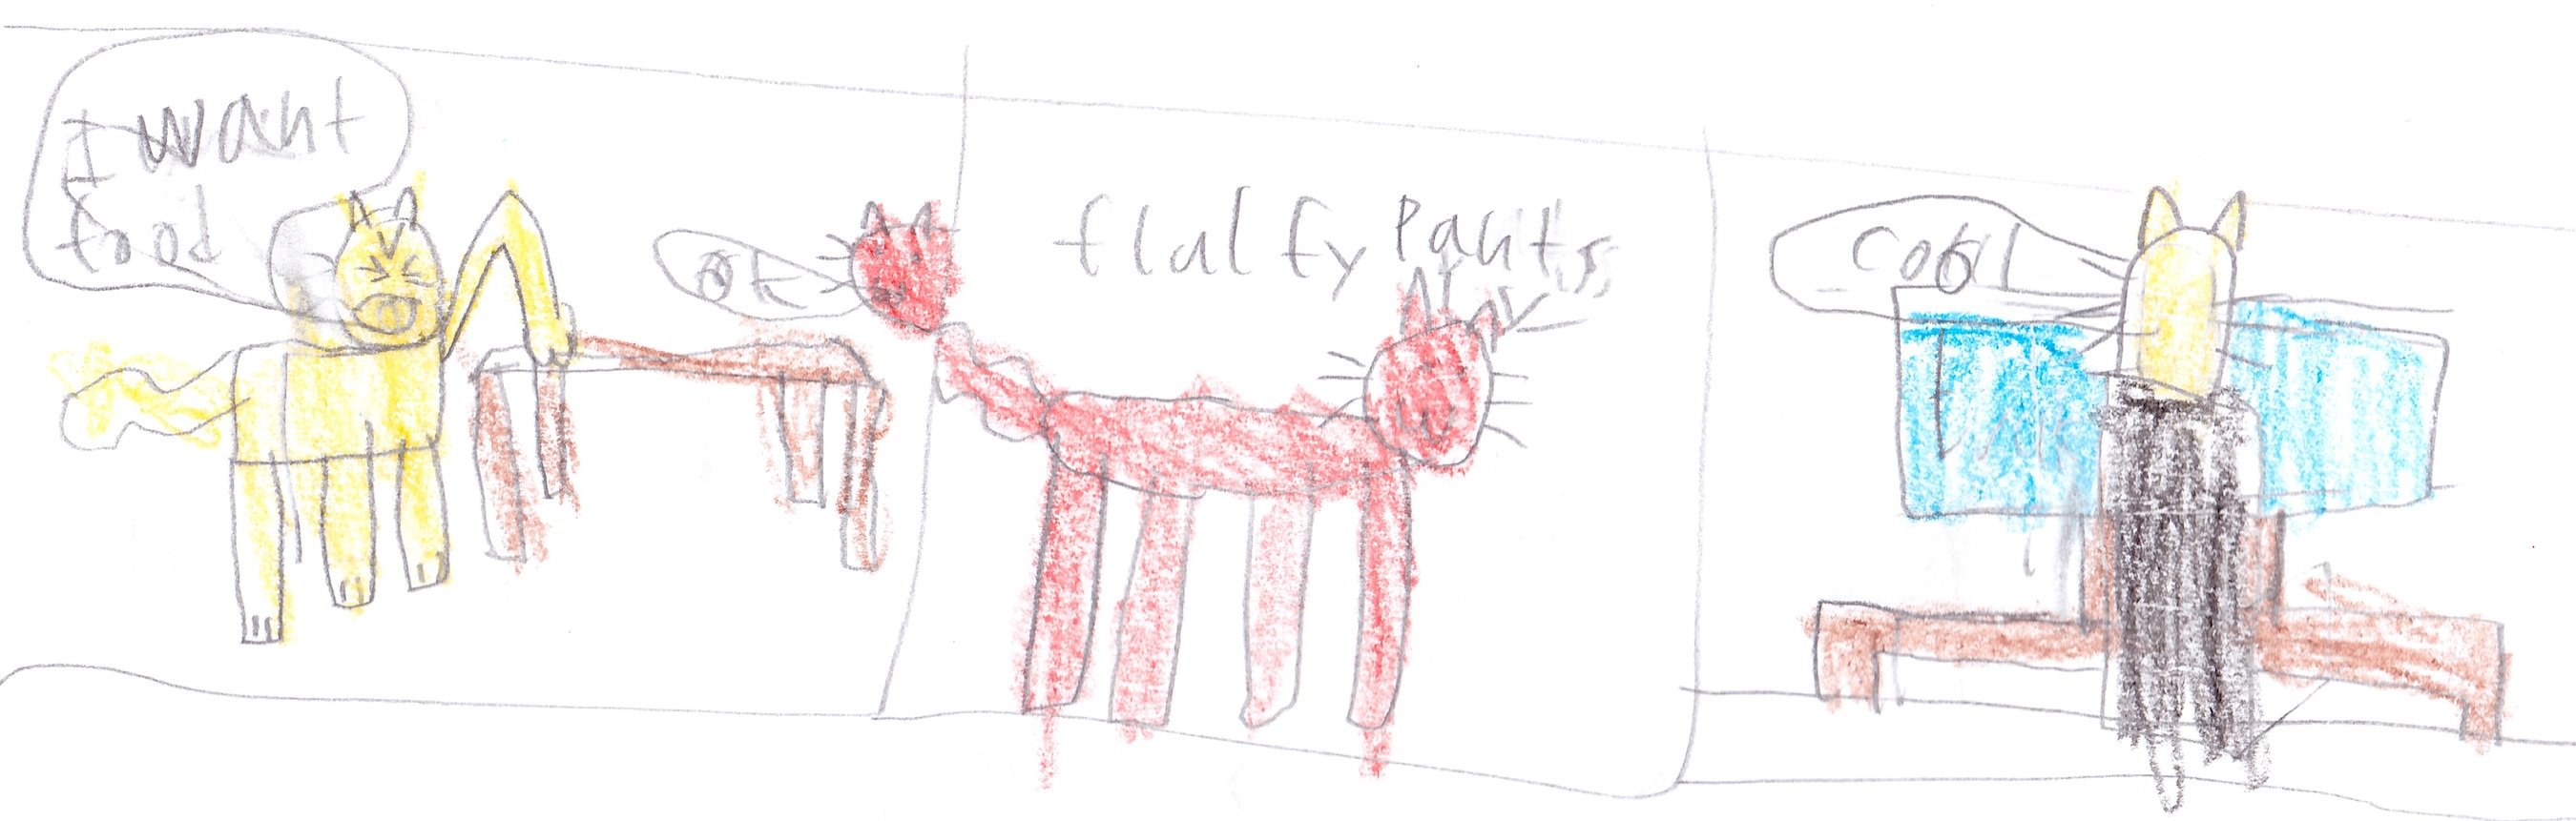
\includegraphics{img/fluffypants.jpg}

7:00 o'cat KM (7 AM): King Cat woke up he walked down the stairs. He
looked at his kitchen table it was very dirty which made King Cat very
angry.

He screamed, ``Where's my food! Clean my table!!!''

``Right away sir,'' said his most helpful and polite helper, Mr Fluffy
Pants.

Mr Fluffy Pants was the most kind to King Cat in all of Cat Planet.
After breakfast King Cat sat down and watched the news.

``Come on! Another report about Kitty saving Cat Planet?'' King Cat
said.

King Cat was about to change the channel when he saw something shiny.

``Very interesting\ldots{}'' said King Cat.

\hypertarget{the-big-crystal}{%
\chapter{The Big Crystal}\label{the-big-crystal}}

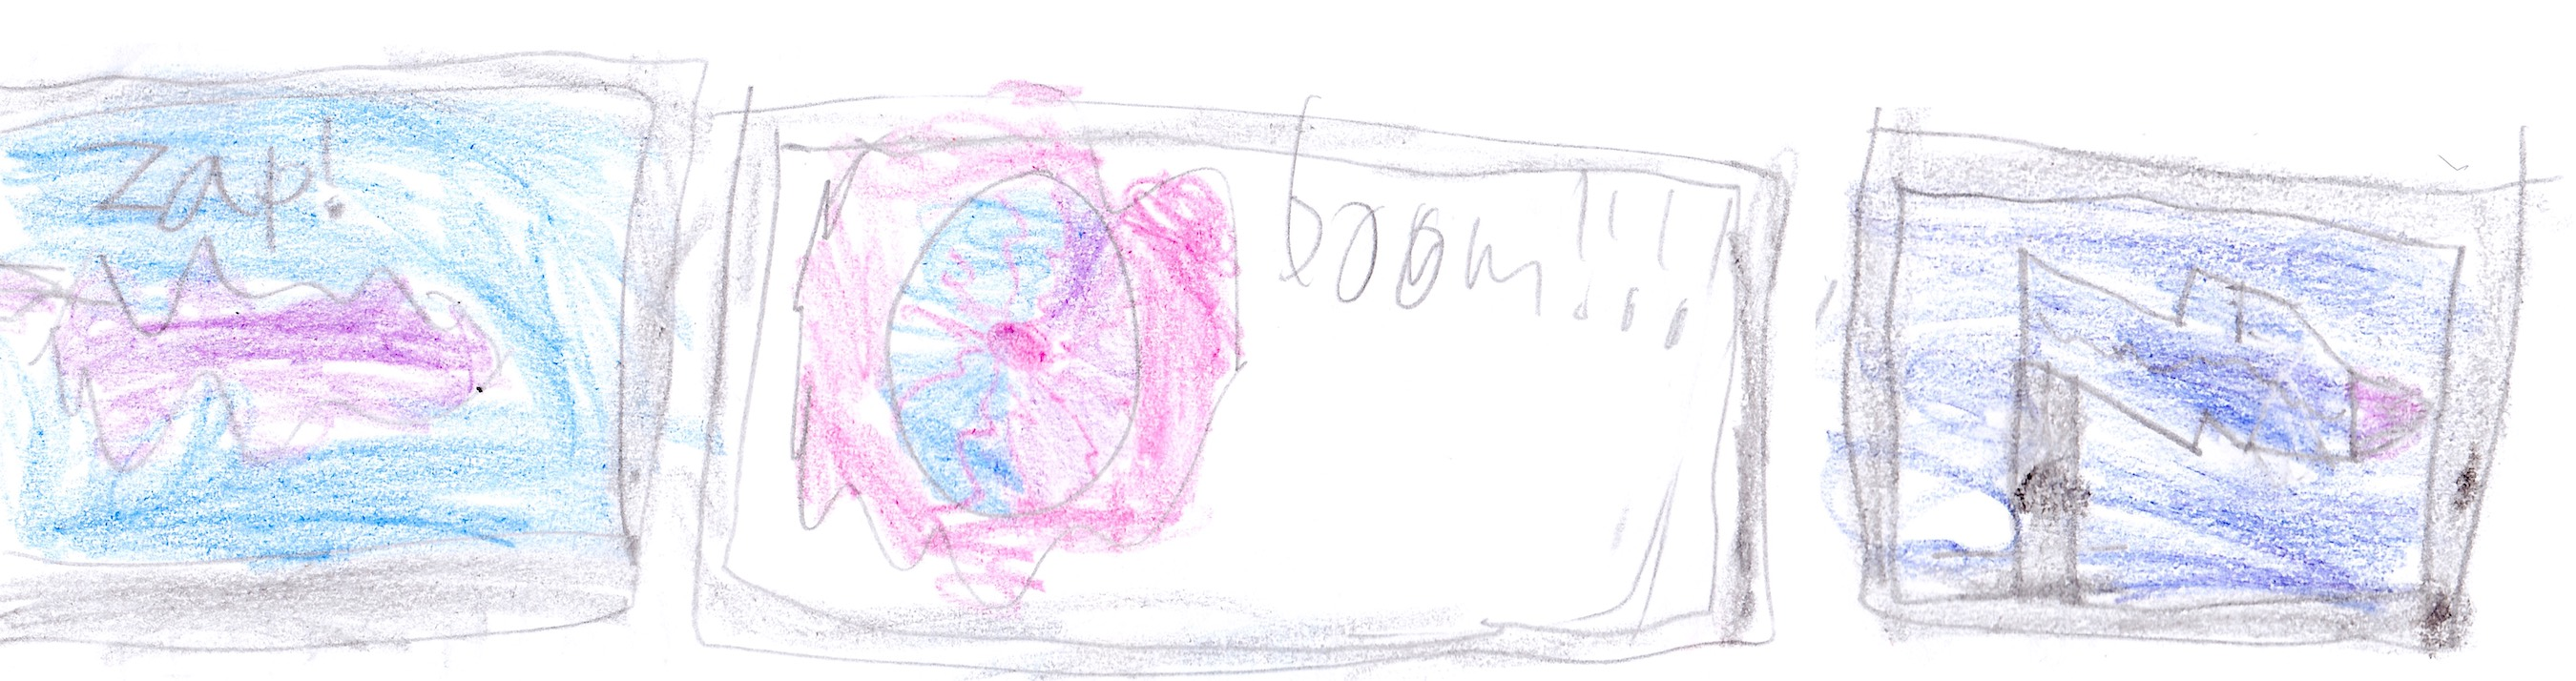
\includegraphics{img/boom.jpg}

The reporter said, ``Hi, I am reporter Fish (a common cat name on Cat
Planet). Today we are honoring Kitty for defeating Super Cat.
Unfortunately he got away as always. Now we will be giving an interview
on Kitty.''

``Thank you, Fish.'' said Kitty.

``The bad guys were going to use Miss Crystal to shoot a very powerful
blast of energy. Here's some pictures by Beckett and Felix to show you
what would happen. But before they did that I went in and POW! WACK!
BLAM! and got the crystal.''

``You explain that very well,'' said Fish.

``Goodbye, everybody!''

King Cat turned off the TV and said, ``I have a plan to get Kitty put in
jail. Hahaha!''

\hypertarget{the-plan}{%
\chapter{The Plan}\label{the-plan}}

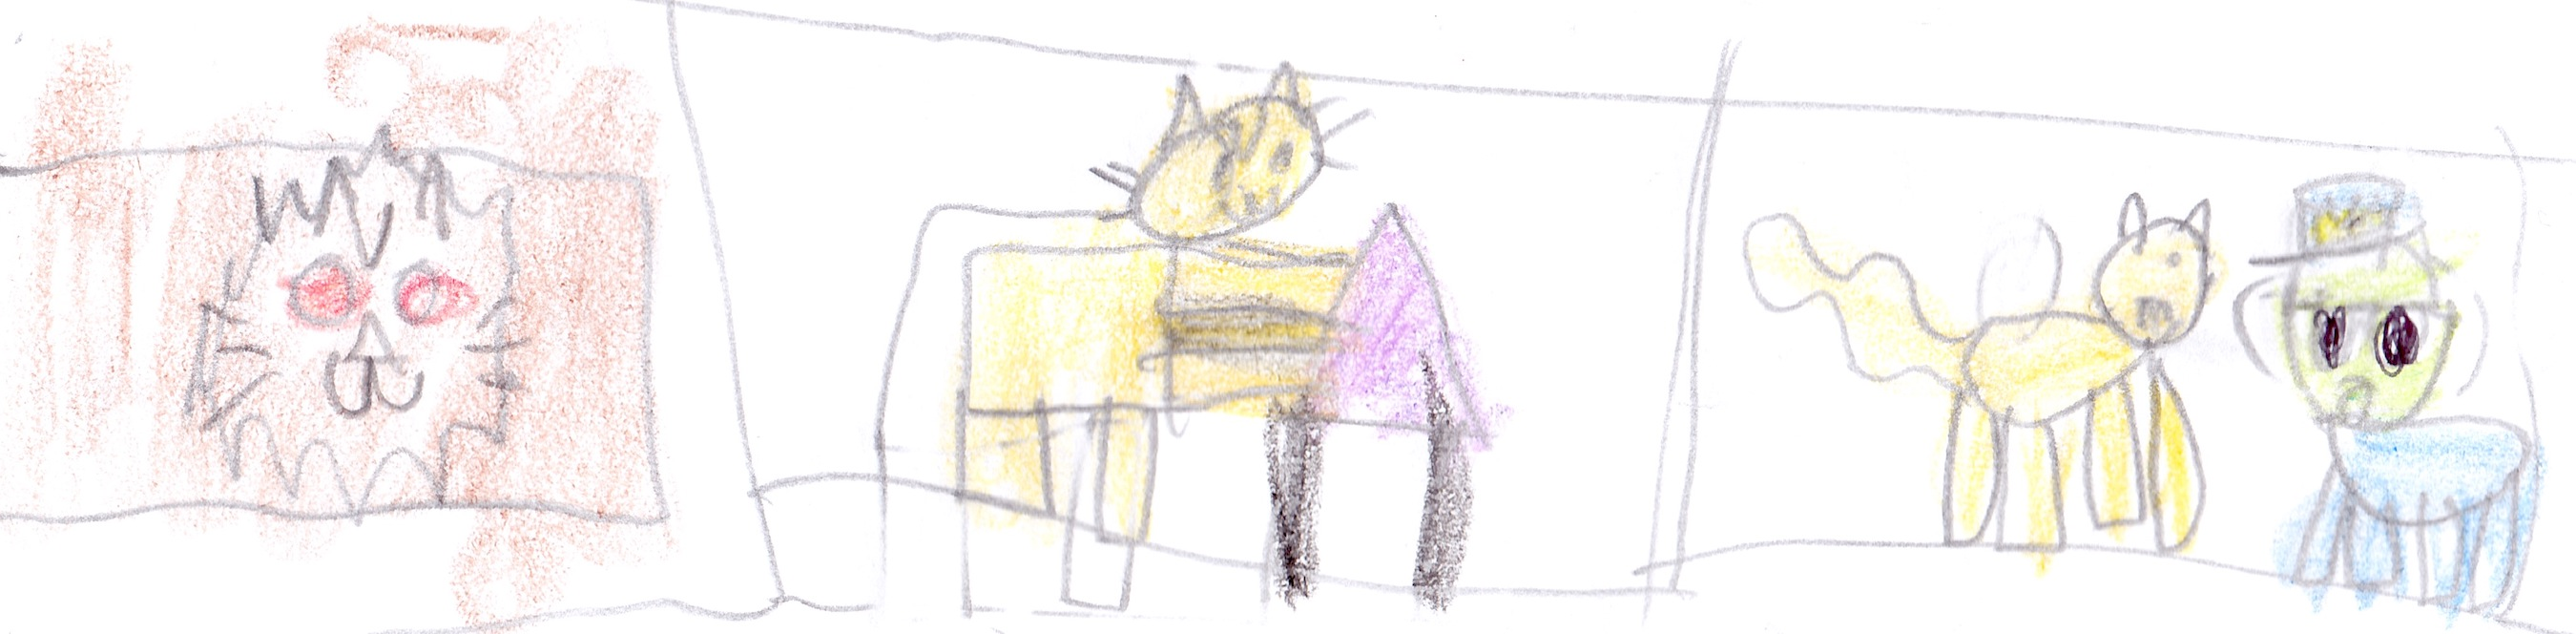
\includegraphics{img/cattriangle.jpg}

``I will go into Kitty's house and steal his crystal and then Kitty and
I will go to court where I can put him in jail,'' King Cat said.

10:30 o'cat KM (10:30 AM): Kitty was on a mission when King Cat broke in
Kitty's house. He grabbed the crystal. He got out the door when the cops
were there.

The cops said, ``You and Kitty are going to court.''

\hypertarget{the-trial}{%
\chapter{The Trial}\label{the-trial}}

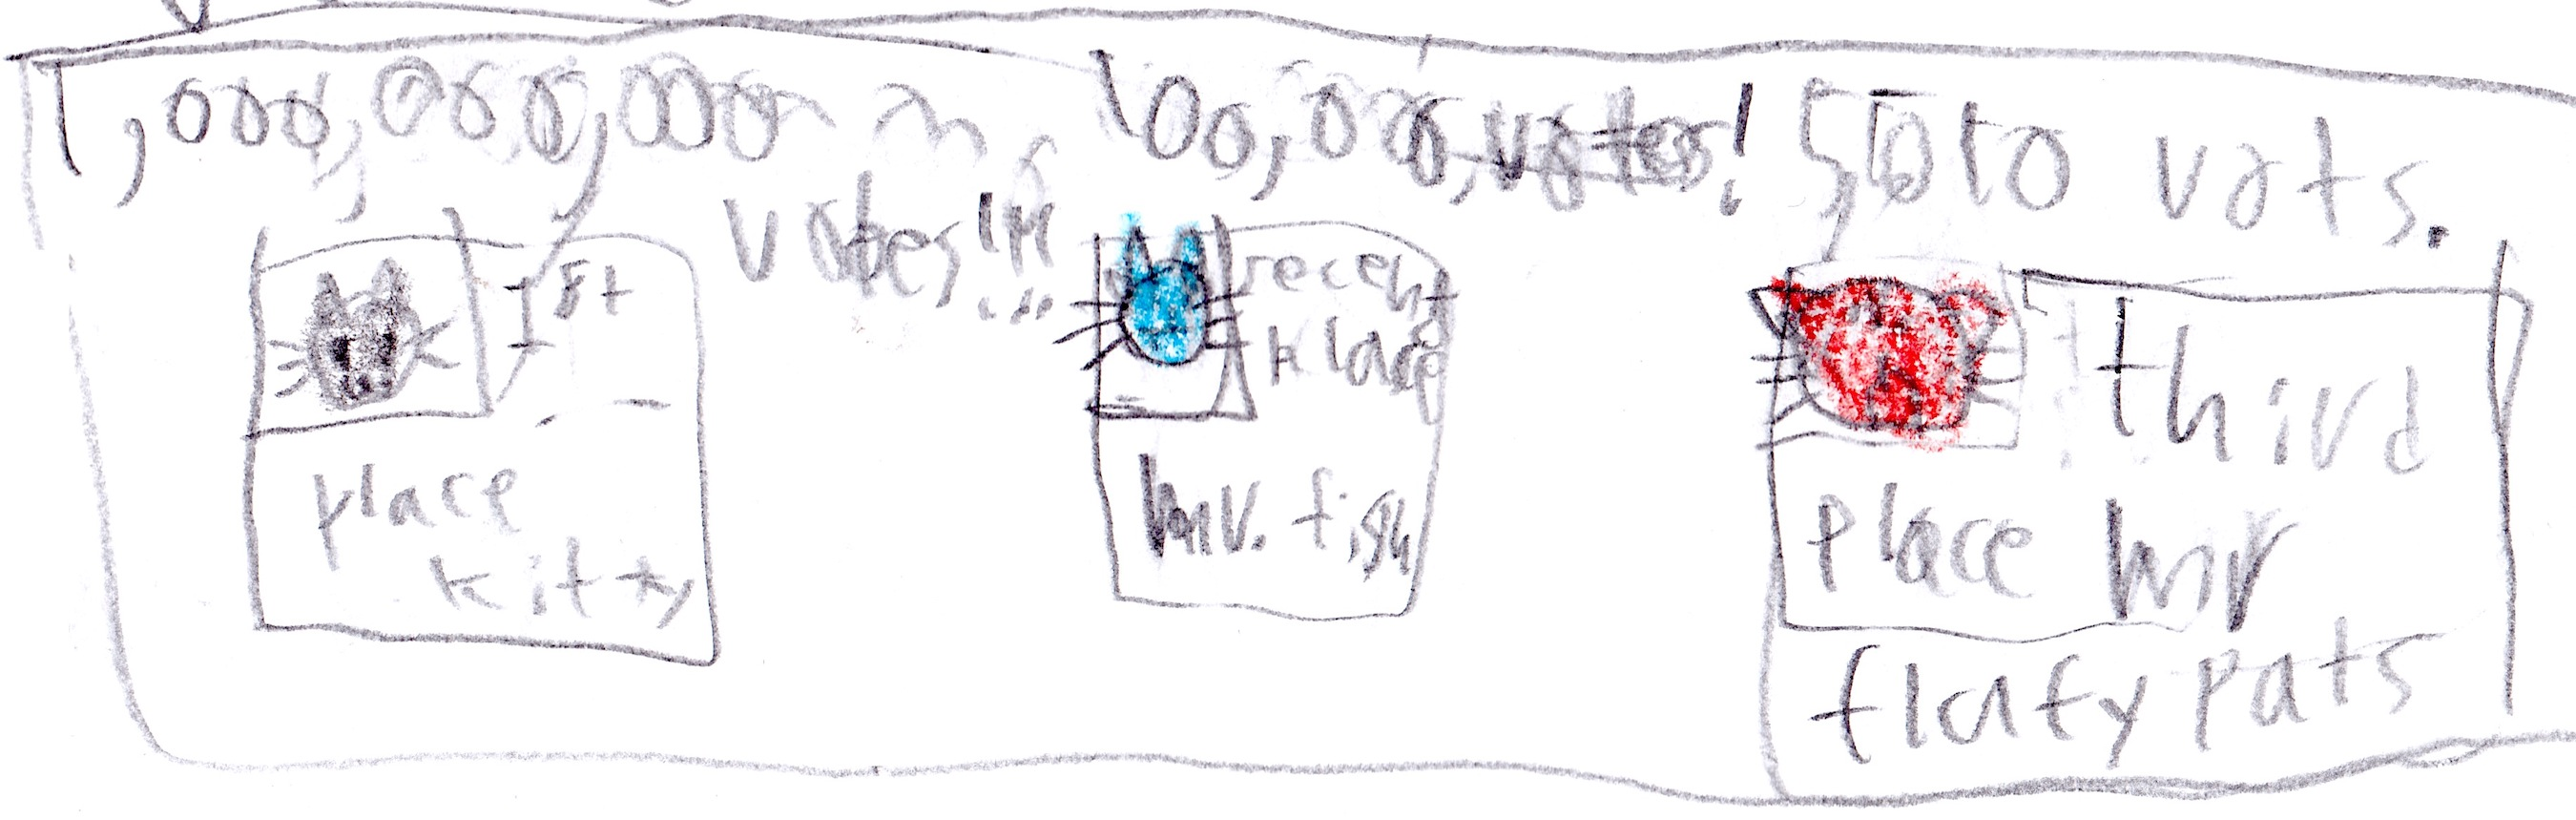
\includegraphics{img/thirdplace.jpg}

Kitty and King Cat are in court. Kitty said, ``King Cat stole the
crystal. I know you know that.''

Everybody did know that.

King Cat said, ``Kitty is going to jail and anybody who tries to stop me
will go to jail too!''

The people did not want to be kicked in jail but guards grabbed Kitty by
the tail and were about to put him in jail.

Kitty said ``Stop! Hear me out! King cat is a monster. He is controlling
you. It's now or never! Throw King Cat out of Cat Town.''

``What?!'' King cat said.

The cats let go of Kitty and grabbed King Cat and threw him out of Cat
Town.

\hypertarget{a-new-king}{%
\chapter{A New King}\label{a-new-king}}

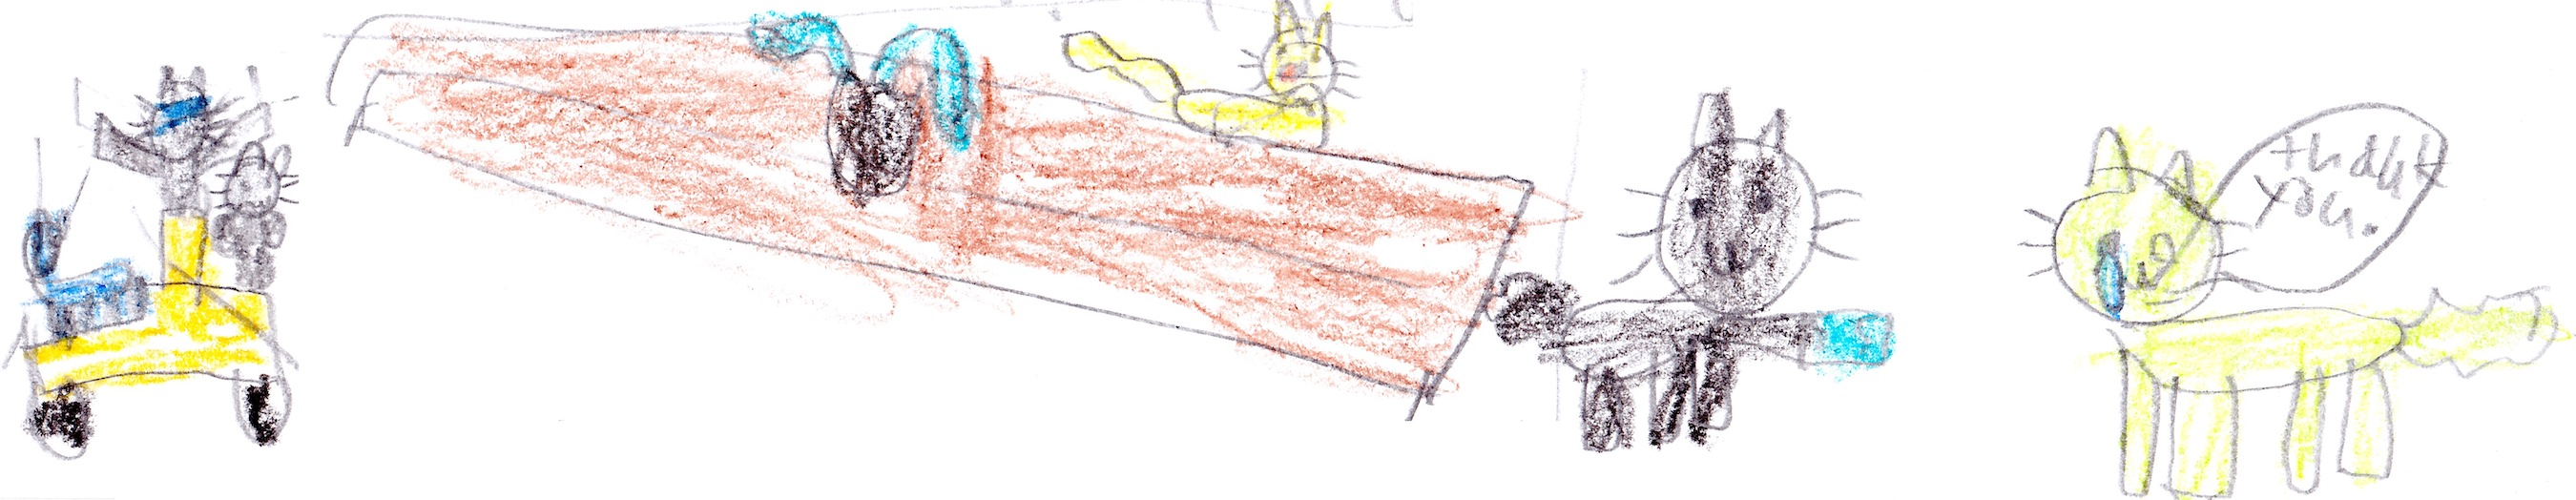
\includegraphics{img/thankyou.jpg}

Right away people started voting for a new king. Kitty won by far. That
night Kitty opened the castle pier. Every cat got to eat a big fish
dinner. Some of the people cried for joy.

They said, ``Oh man! He gave us fish! He gave us tons of tuna and
salmon!''

Kitty said, ``Glad you enjoyed my free fish dinner.''

They said, ``It's free?! It's free!!'' and they walked away happy.

9:00 o'cat FM (9 PM): Kitty chose new helpers. The top two were Grace
and Fluffy. The next day Kitty gave five cat dollars to every cat that
was in a parade.

``Kitty is the best ever!'' the audience shouted.

But every big event with Kitty only made King Cat madder and madder.

King Cat said, ``I have to get my revenge on Kitty but I need another
helper.''

``I know just the one,'' Mr Fluffy Pants said.

\hypertarget{super-cat}{%
\chapter{Super Cat}\label{super-cat}}

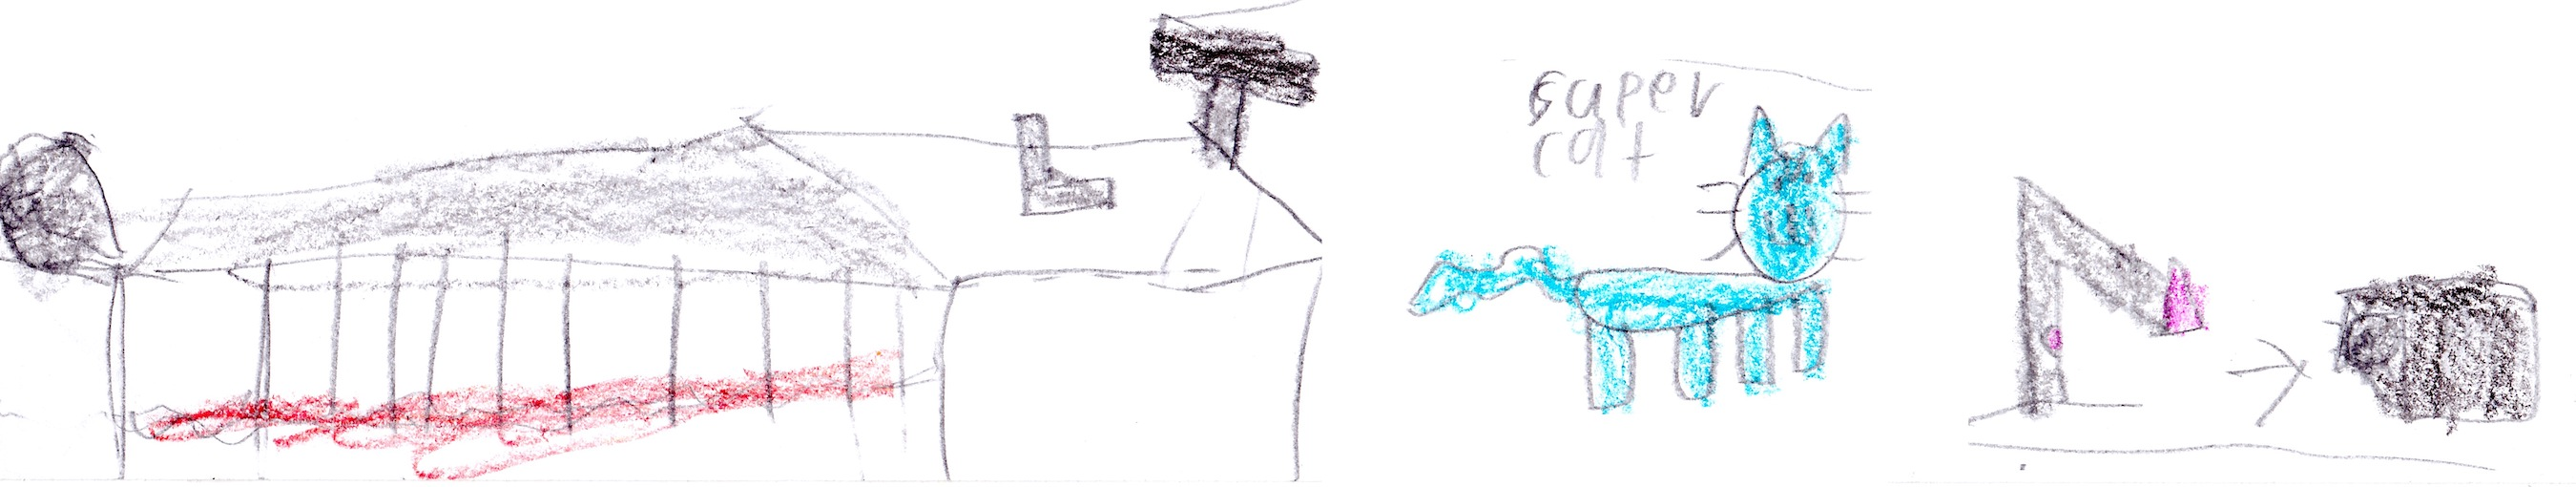
\includegraphics{img/supercat.jpg}

King Cat followed Mr Fluffy Pants until Mr Fluffy Pants stopped at a
mountain.

King Cat frowned and said, ``This isn't a base.''

Then Mr Fluffy Pants put his hand on the side of the mountain. A secret
passage opened up. They walked inside. The door closed. They stopped in
a room that had a big bridge and lava around the bridge. This isn't the
bridge in the books that falls apart easily. They walked on the bridge
and then heard a hiss. Somebody got out the chair. It was Super Cat.

``Super Cat how is it going?'' Mr Fluffy pants asked.

Super Cat said, ``Horrible. I need that crystal.''

Mr Fluffy pants handed the crystal over to Super Cat.

``You know you are the only one who can escape Kitty, but together we
can defeat Kitty. Join us, Super Cat!'' Mr Fluffy Pants said.

``OK'' said Super Cat.

Super Cat put the crystle in the machine called the Laser Ray 2000 and
pressed a button that transformed it into a little box.

Super Cat said, ``It can't destroy the wall, it can only destroy a big
building.''

``How about Kitty's Castle?'' said King Cat.

\hypertarget{the-destruction-of-cat-planet}{%
\chapter{The destruction of Cat
Planet}\label{the-destruction-of-cat-planet}}

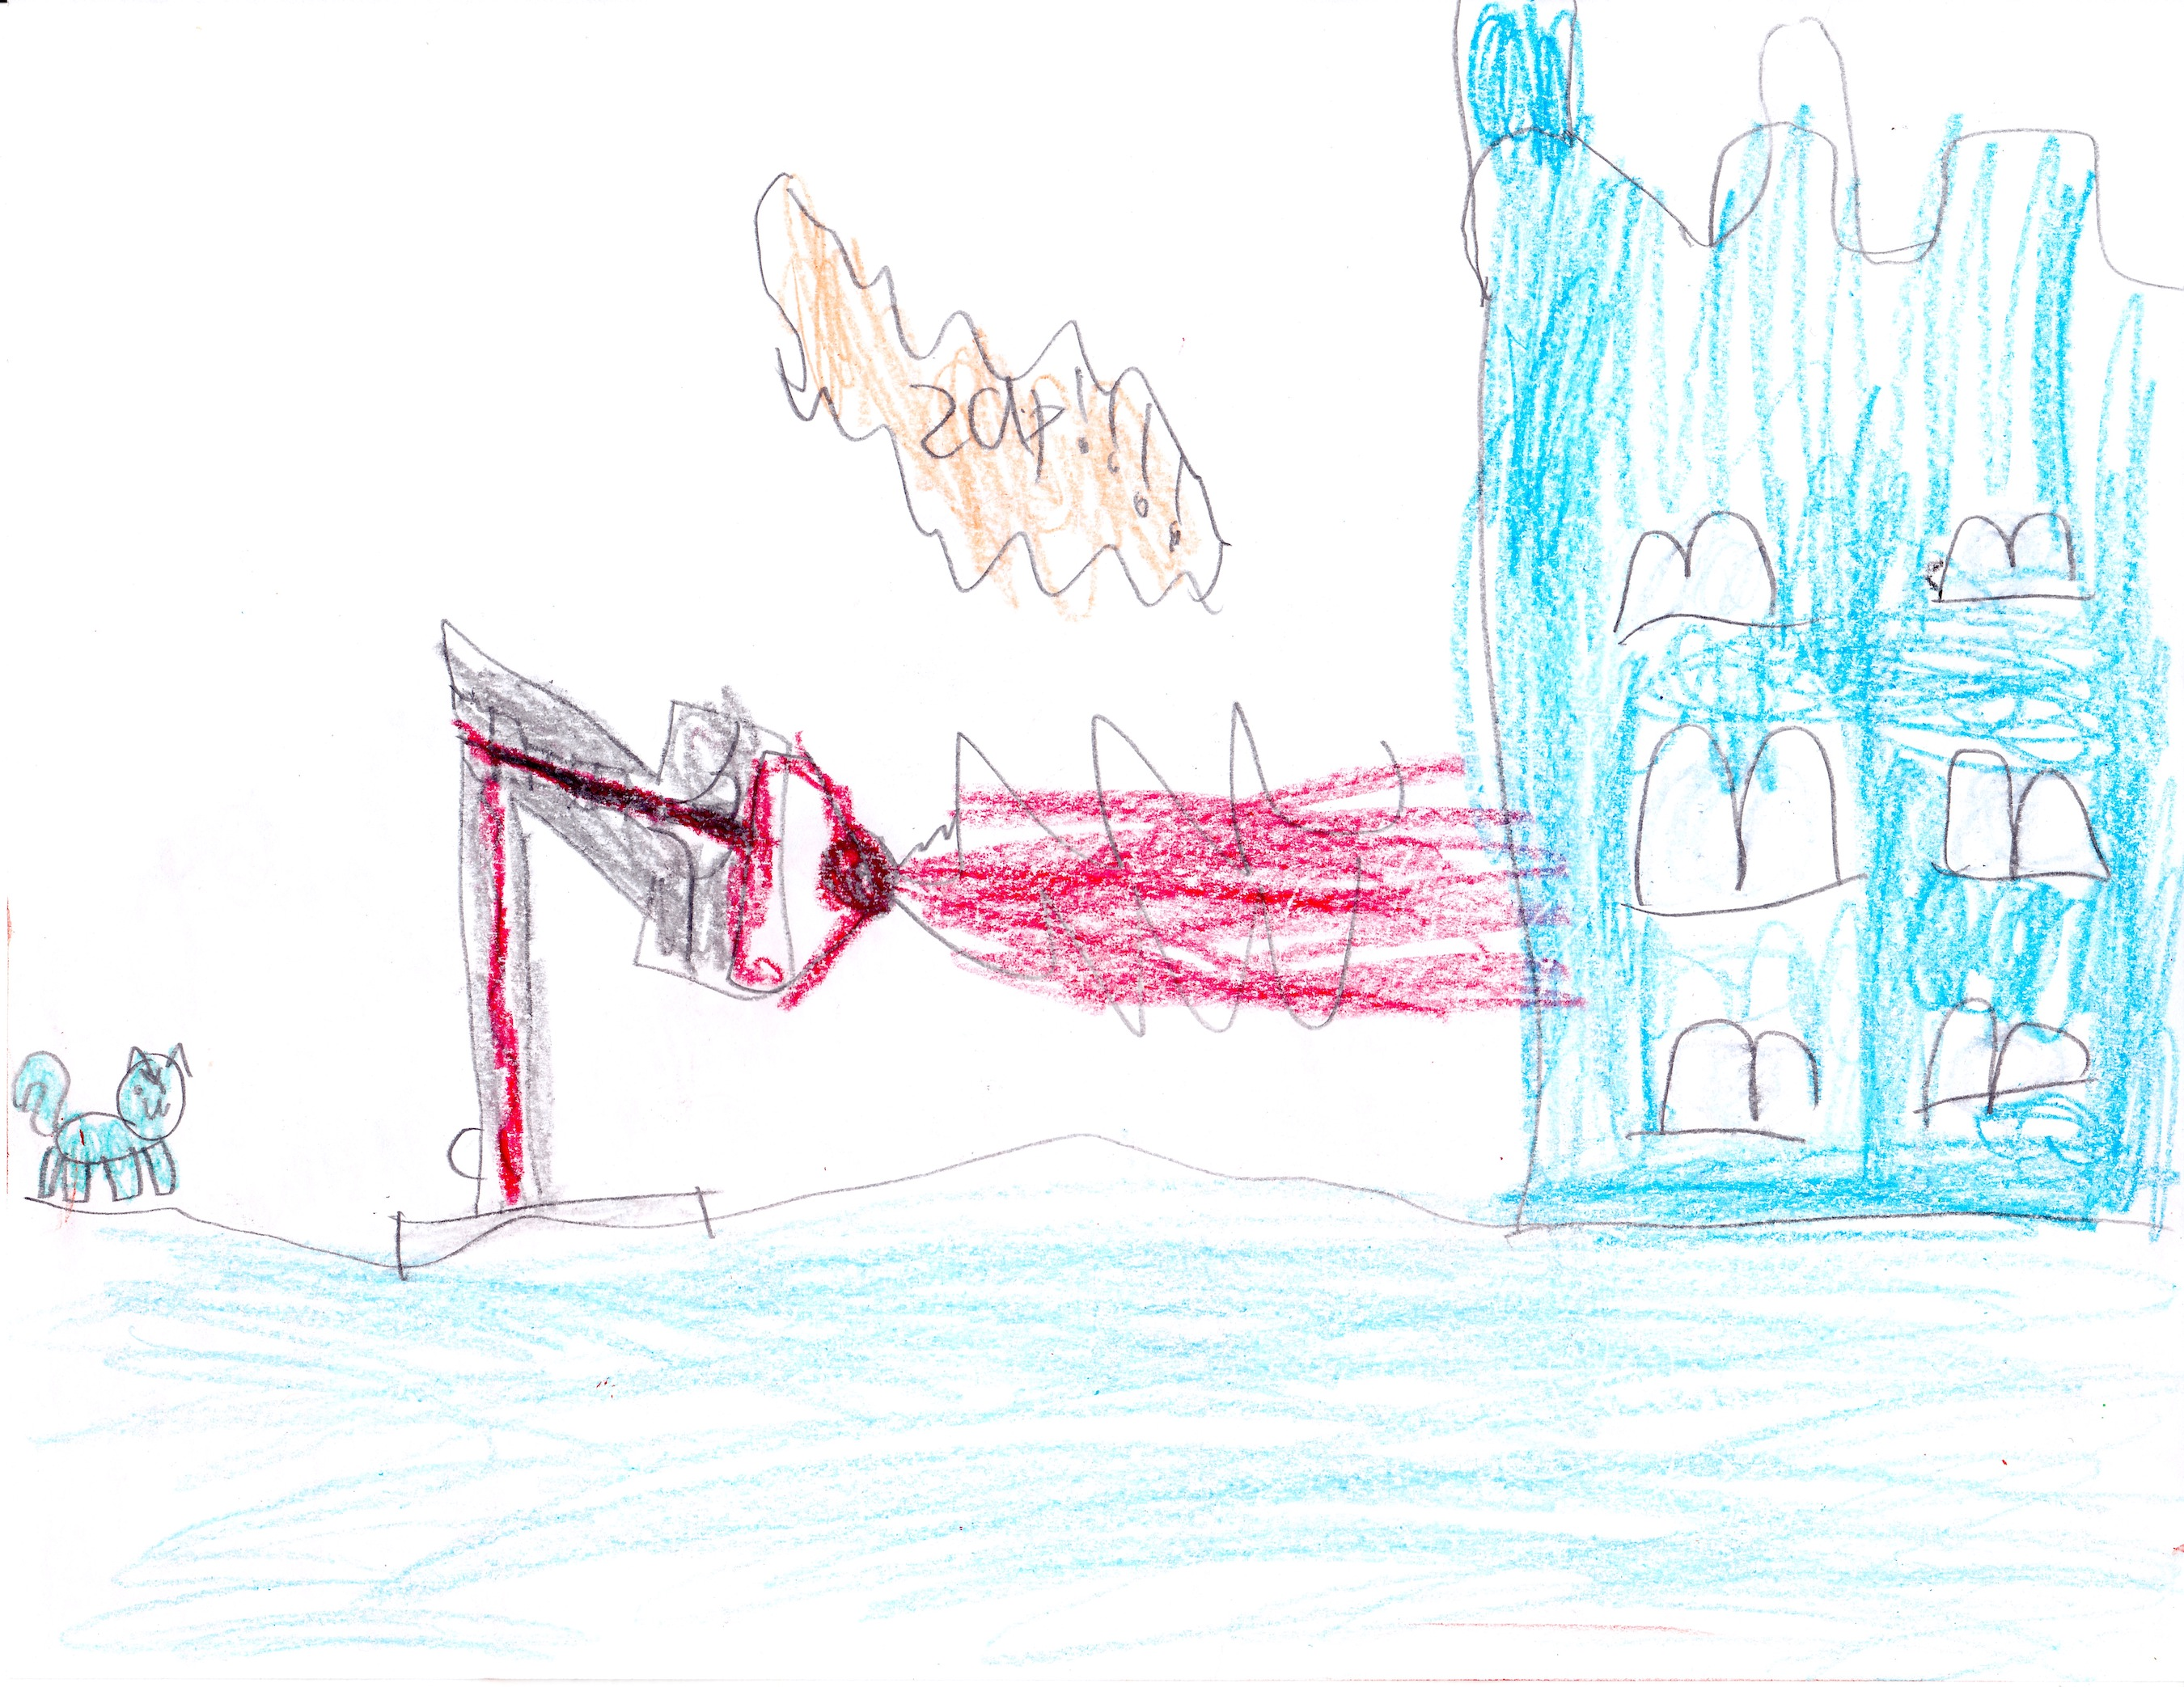
\includegraphics{img/laser.jpg}

The next morning Kitty woke up. People were running, so Kitty ran and
opened the door. Super Cat shot the laser and destroyed Cat Castle.
Everyone died. Only Kitty, Grace, and Fluffy survived. But Cat Planet
was cracking.

``Wow!'' Kitty said.

``It can't be \ldots{} Cat Planet is exploding! Let's get out of here!''
Super Cat said.

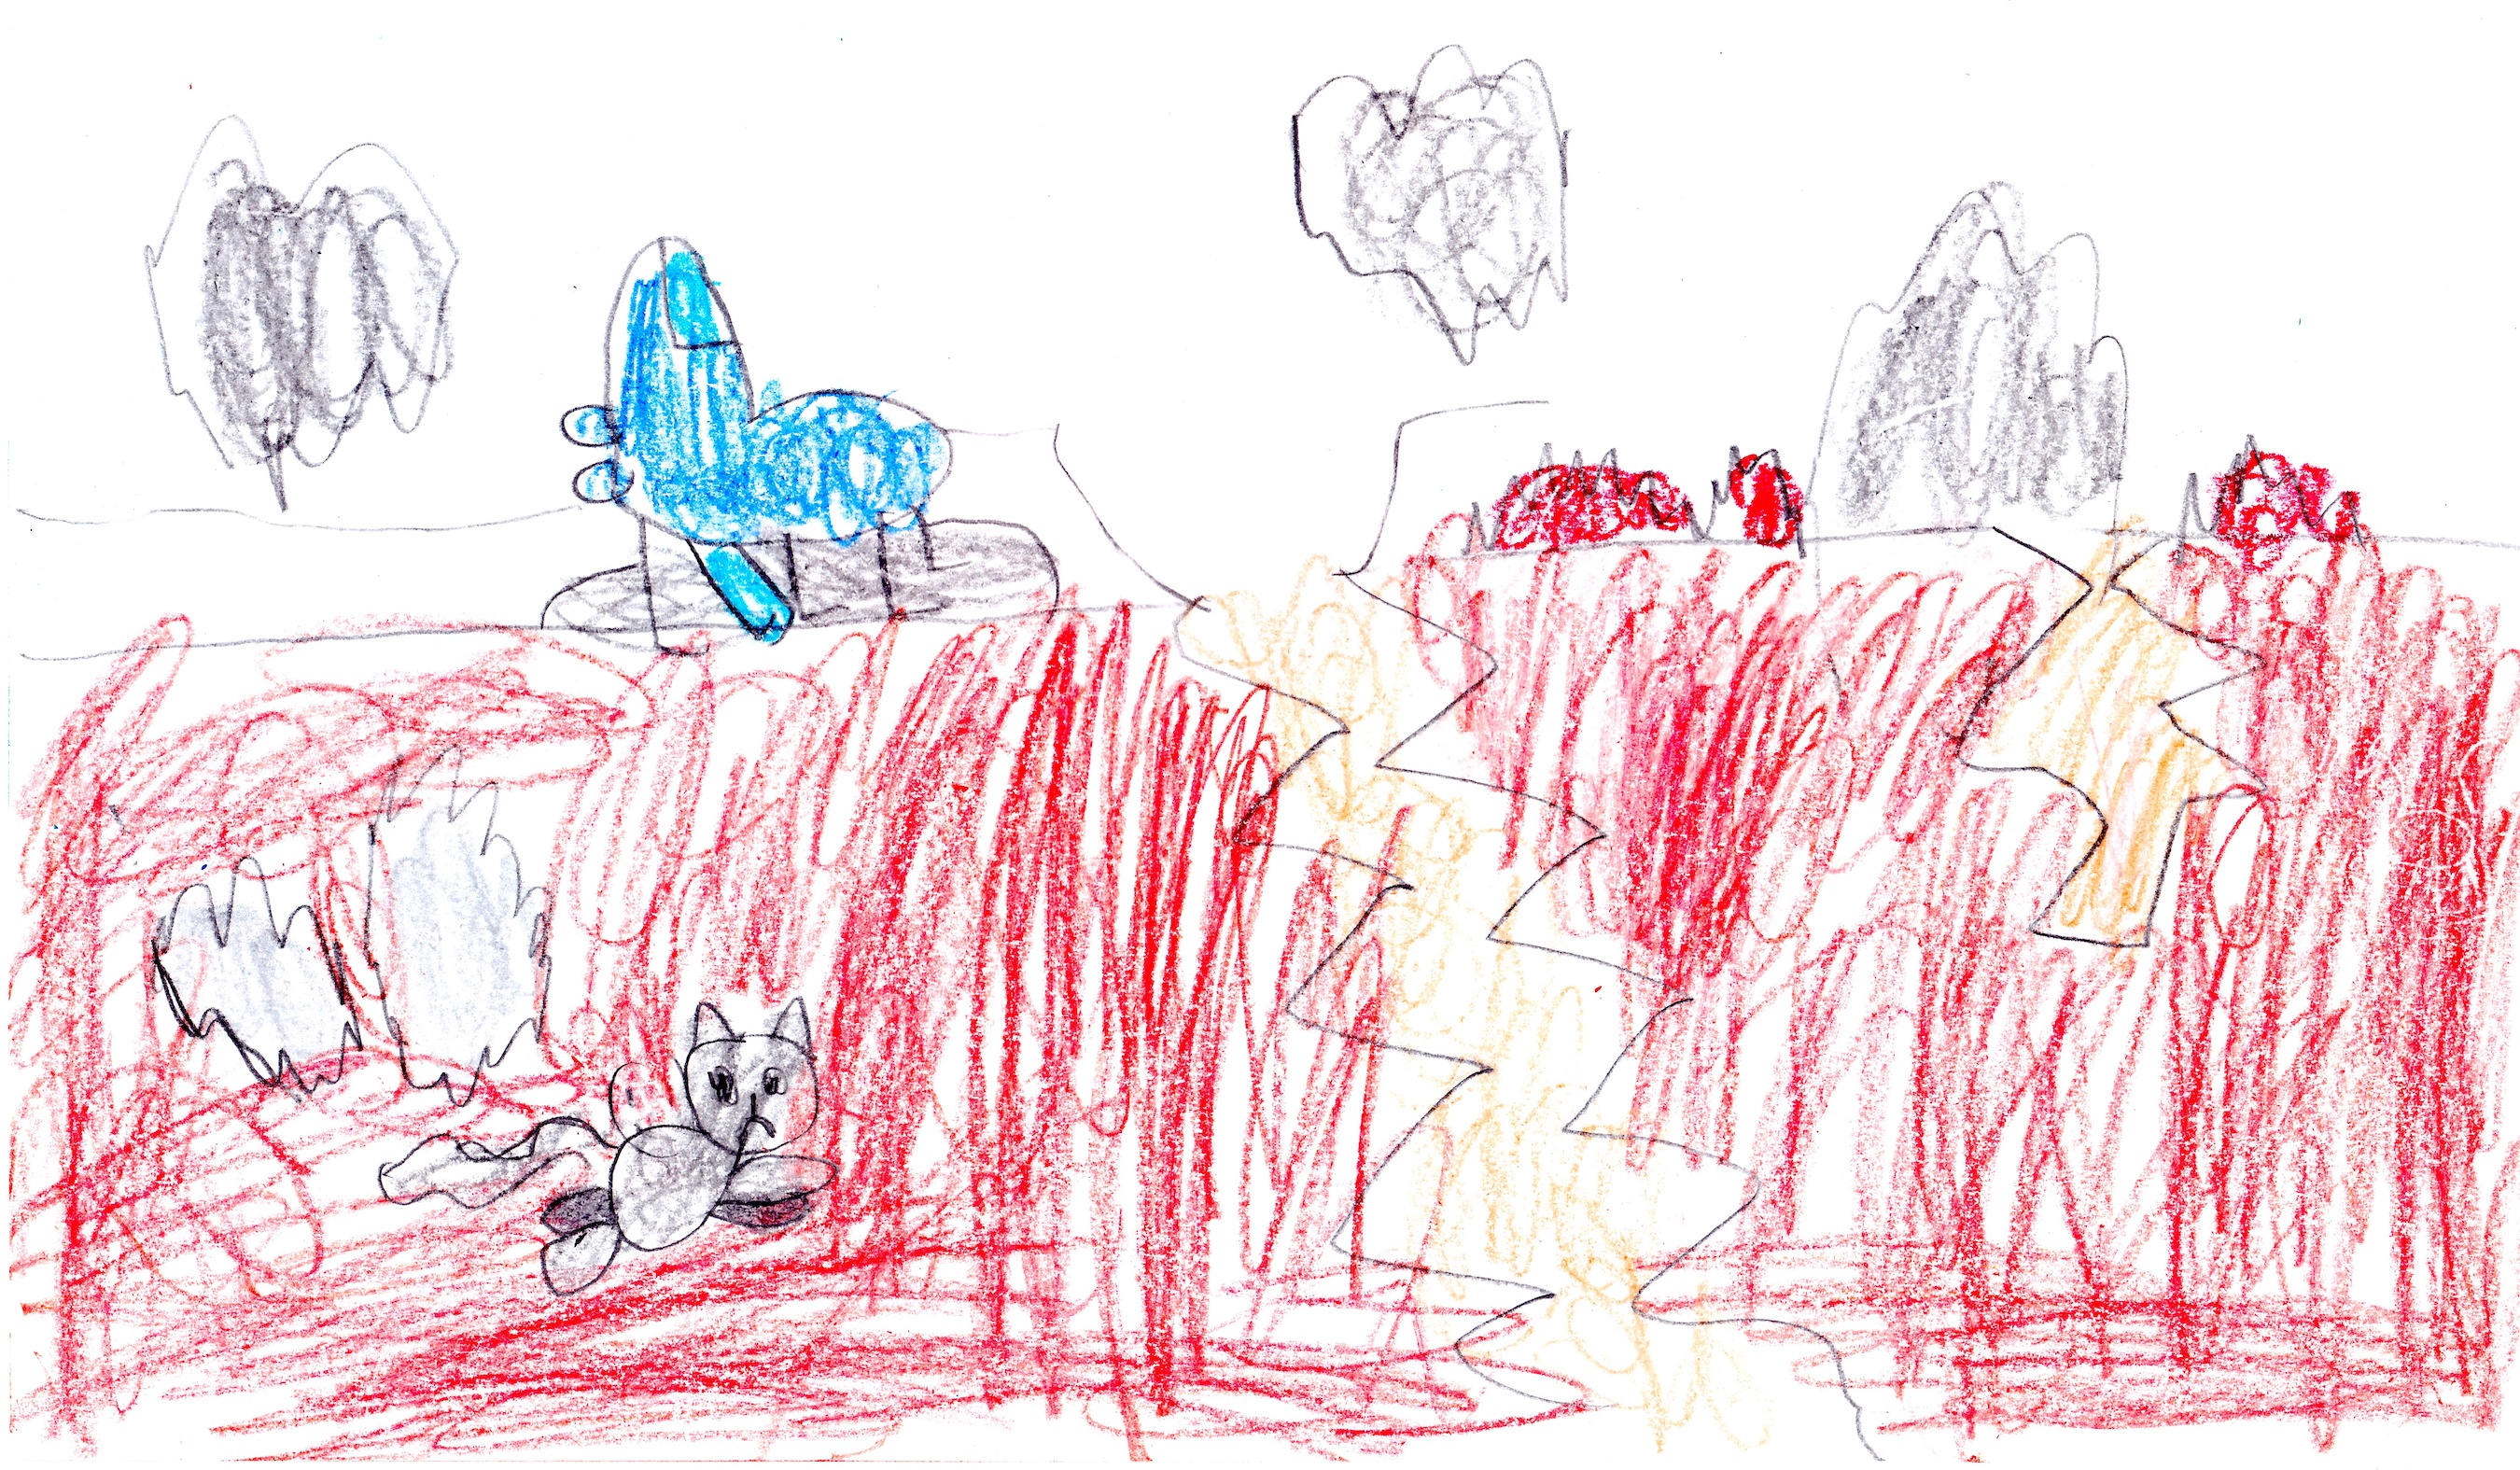
\includegraphics{img/lava.jpg}

They got in a spaceship. Super Cat took one while King Cat and Mr Fluffy
Pants took another. The two purple ships flew out of Cat Planet. Kitty
got Fluffy and Grace then put them in a small blue ship. They flew away
also as bits of rocks and pebbles left the planet.

BANG!!!

Cat Planet was destroyed and the only remaining survivors were Super
Cat, King Cat, Mr Fluffy Pants, Kitty, Grace, and Fluffy.

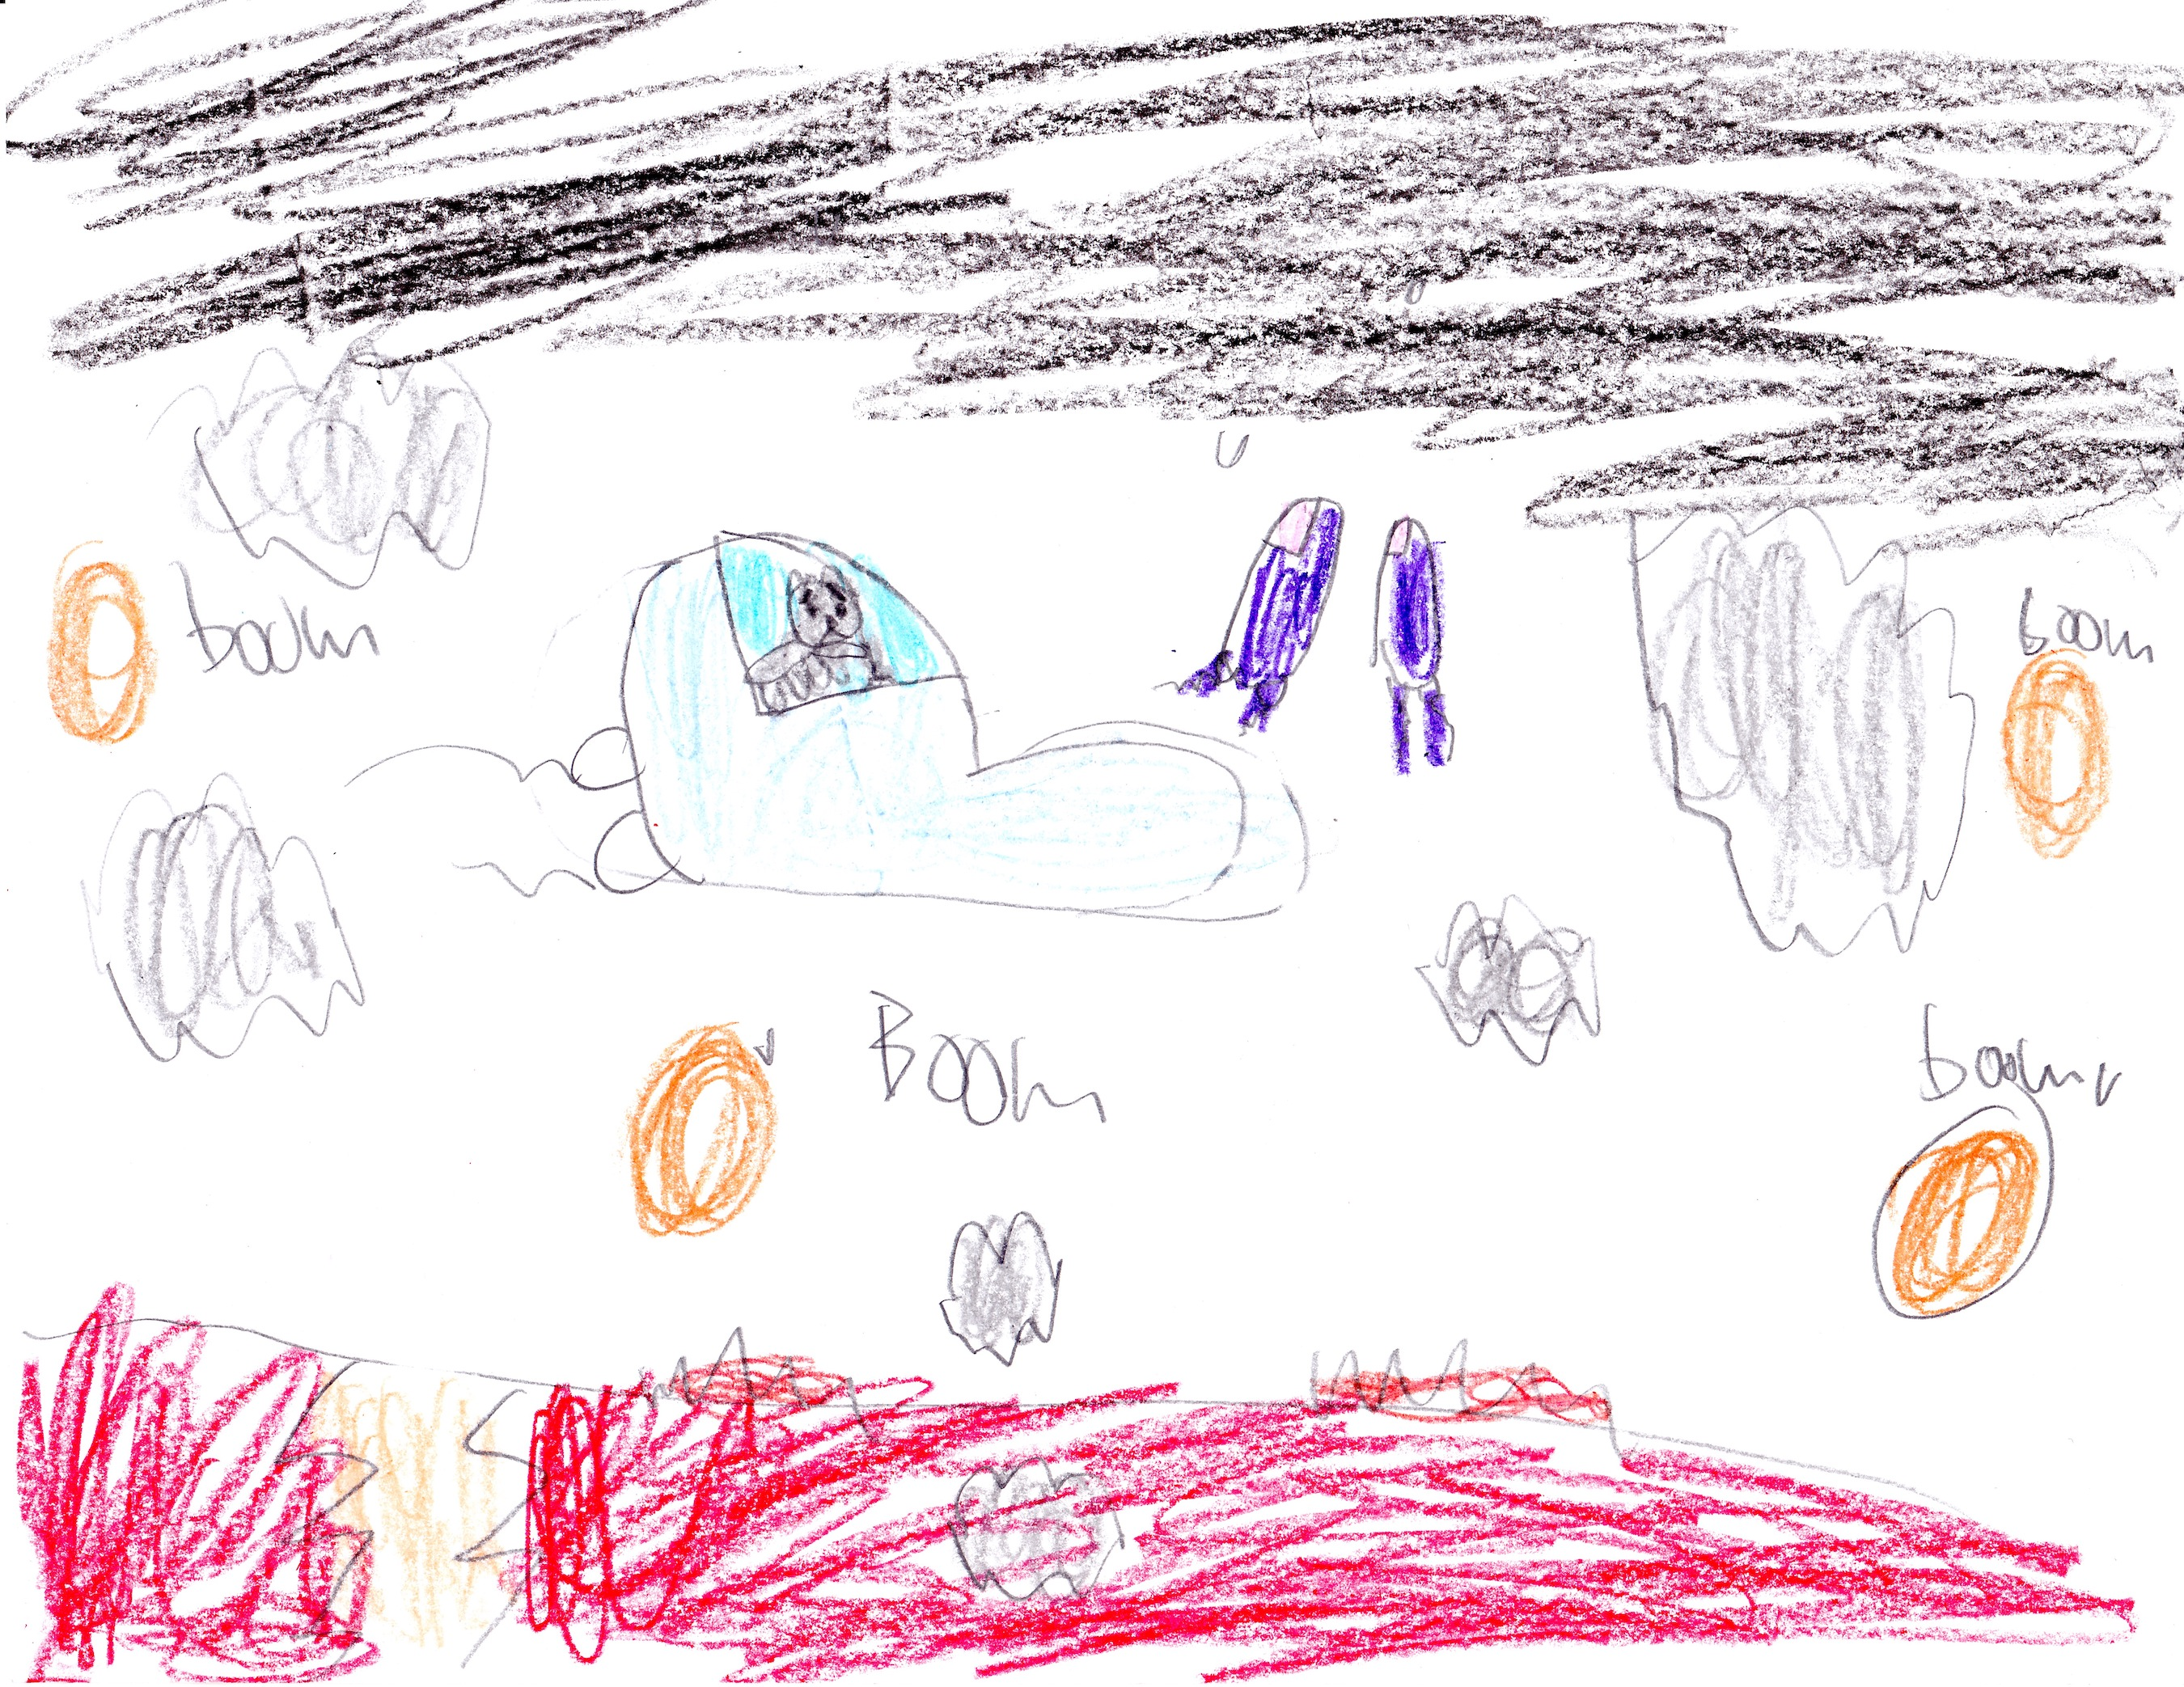
\includegraphics{img/flying.jpg}

\end{document}
